\chapter{\label{chap:szenarien}Szenarien im Ampelbereich}
Alle in Kapitel \ref{chap:state} angeführten Studien zu Ampelinformationssystemen und Konzepte zu Fahrraderweiterungen haben die Gemeinsamkeit des selbstkontrontollierten Fahrverhaltens der FahrerInnen. Ausgesprochen werden lediglich Empfehlungen, die möglichst intuitiv und schnell vermittelt werden. Grundlegend sollte die Anwendung in der Lage sein, die passende Empfehlung oder Handlungsaufforderung anzuzeigen, die sich aus folgenden Szenarien ergeben.
\begin{figure}[H]  
    \centering  
    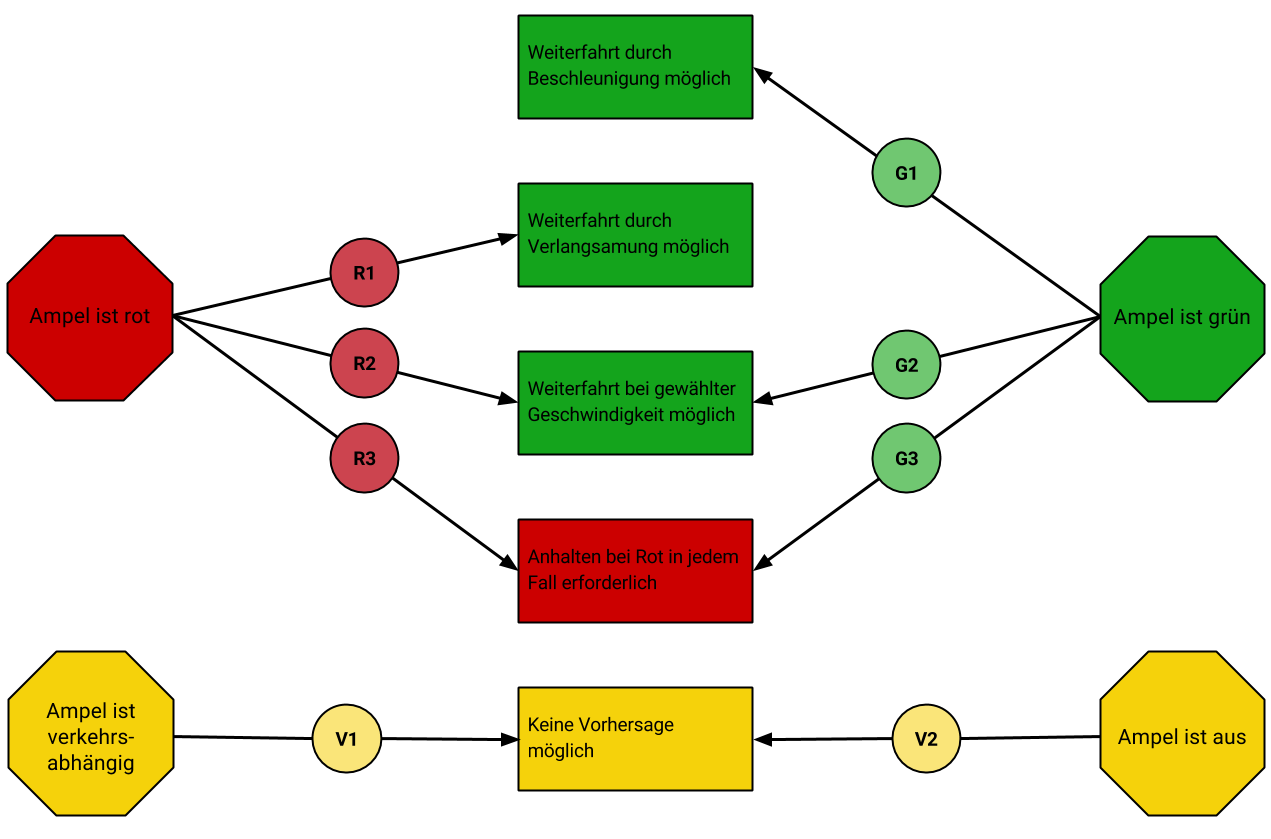
\includegraphics[width=1\textwidth]{Szenarien} 
    \caption[Szenarien]{Szenarien im Ampelbereich}
    \label{fig:szenarien}
\end{figure}
\begin{description}[leftmargin=0.7cm,style=nextline]
\item[Szenario R1:] 
Zeigt die Ampel im Moment und noch eine ganze Weile auf Rot ist je nach Distanz zwischen Ampel und Fahrrad ist ein reibungsloses Passieren der Ampel durch Beschleunigung oder ohne Änderung der Geschwindigkeit zu erreichen.\\
\item[Szenario R2:] 
Die Ampel zeigt im Moment auf Rot, aber die Restrotzeit ist kurz. Auch hier gilt: Je nach Entfernung zwischen Fahrrad und \gls{LSA}, ist ein reibungsloses Passieren der Ampel durch Verzögerung oder ohne Änderung des Tempos zu erreichen.\\
\item[Szenario R3:] 
Zeigt die Ampel im Moment Rot, die Restrotzeit ist lang, doch die Entfernung zwischen Fahrrad und \gls{LSA} hoch, so ist keine Weiterfahrt ohne Unterbrechung möglich.\\
\item[Szenario G1:] Ist die empfohlene Geschwindigkeit gleich der aktuellen, ist ein reibungsloses Passieren bei beibehaltenem Tempo möglich. Es besteht kein Aktionsbedarf.\\
\item[Szenario G2:] 
Zeigt die Ampel im Moment Grün und ist die empfohlene Geschwindigkeit höher als die aktuelle, ist ein reibungsloses Passieren durch Beschleunigung zu erreichen. Bei der Anzeige der Progressionsgeschwindigkeit ist selbstverständlich die geltende Höchstgeschwindigkeitsbegrenzung oder die eingestellte Höchsteschwindigkeit zu beachten.\\ 
\item[Szenario G3:] 
Zeigt die Ampel im Moment Grün und ist die empfohlene Geschwindigkeit höher als die aktuelle und gleichzeitig auch höher als die zugelassene, bzw. eingestellte Höchstgeschwindigkeit, ist die Distanz zur Ampel zu groß und ein reibungsloses Passieren nicht möglich.
\end{description}
Resultierend aus den Szenarien im Ampelbereich ergeben sich die folgenden Systemzustände.
\begin{itemize}
	\item Zustand a: Keine Weiterfahrt ohne Unterbrechung möglich
	\item Zustand b: Kein Aktionsbedarf
	\item Zustand c: Weiterfahrt durch Verlangsamung möglich
	\item Zustand d: Weiterfahrt durch Beschleunigung möglich
\end{itemize}
Im weiteren Verlauf wird unter anderem beschrieben wie diese Systemzustände in den Designprozess eingebunden werden.
